\documentclass{article}%
\usepackage[T1]{fontenc}%
\usepackage[utf8]{inputenc}%
\usepackage{lmodern}%
\usepackage{textcomp}%
\usepackage{lastpage}%
\usepackage[head=40pt,margin=0.5in,bottom=0.6in]{geometry}%
\usepackage{graphicx}%
%
\title{\textbf{Hospitales sin aspirinas para salvar a infartados}}%
\author{Olgalinda Pimentel R. | opimentel@el{-}nacional.com}%
\date{21/09/2018}%
%
\begin{document}%
\normalsize%
\maketitle%
\textbf{URL: }%
http://www.el{-}nacional.com/noticias/salud/hospitales{-}sin{-}aspirinas{-}para{-}salvar{-}infartados\_252629\newline%
%
\textbf{Periodico: }%
EN, %
ID: %
252629, %
Seccion: %
Salud\newline%
%
\textbf{Palabras Claves: }%
Salud, Sociedad\newline%
%
\textbf{Derecho: }%
2.1, %
Otros Derechos: %
, %
Sub Derechos: %
2.1.1\newline%
%
\textbf{EP: }%
NO\newline%
\newline%
%
\textbf{\textit{Una encuesta entre 49 centros asistenciales y promovida por la Sociedad de Cardiología reveló que la mitad no tiene capacidad de diagnóstico ni para realizar electrocardiogramas}}%
\newline%
\newline%
%
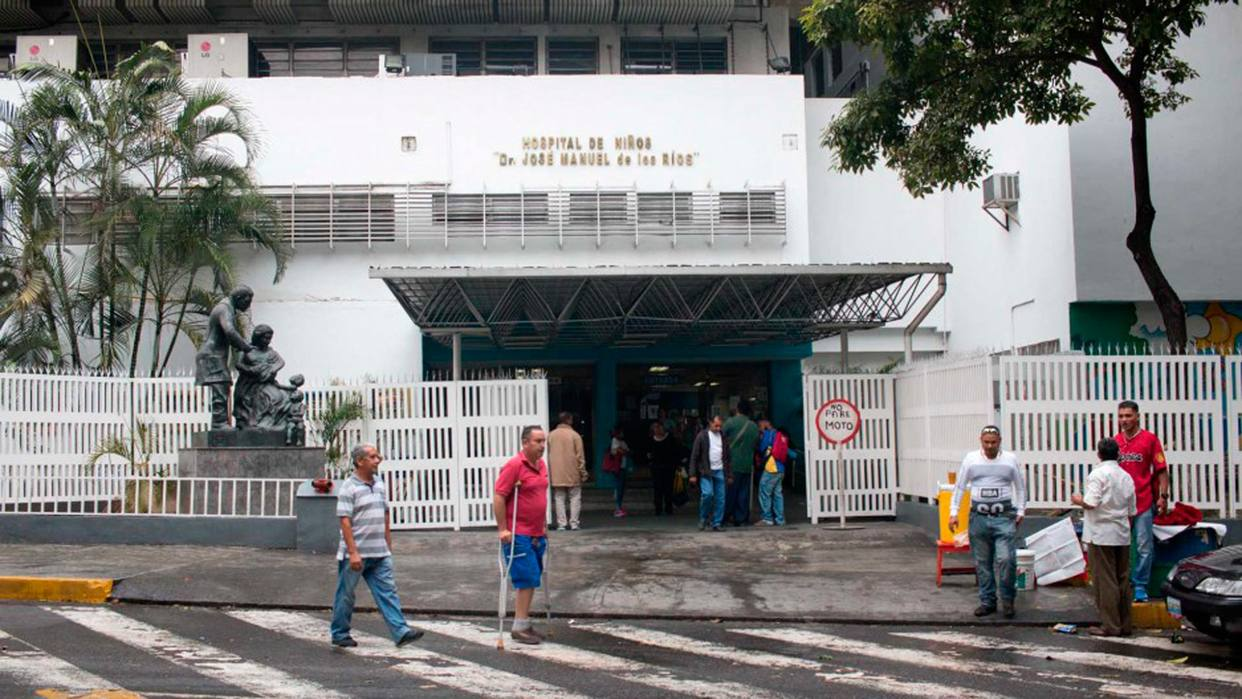
\includegraphics[width=300px]{239.jpg}%
\newline%
%
Una persona con un infarto tiene menos probabilidades que en 2017 de superar la crisis en un hospital venezolano, y ninguna si el evento le ocurre de noche.%
\newline%
%
La Encuesta Nacional de Hospitales realizada en 49 centros de salud públicos, clasificados como 3 y 4, es decir, de referencia, y dependientes del Ministerio de Salud y del IVSS, en el área de cardiopatía isquemia aguda (infartos), determinó que la capacidad de diagnóstico y para realizar electrocardiogramas en los primeros 10 minutos a un paciente que ingresa con dolor torácico, se redujo de 87,5 en 2017 a 59,2\% en 2018; solo 22,4\% de estos centros realizan los procedimientos de día. “De noche no pueden hacer diagnósticos”, afirmó el especialista Carlos Ponte Negretti, directivo de la Sociedad Venezolana de Cardiología y coordinador del estudio “Monitoreo de síndrome coronario agudo 2018”, el cual presentó ayer en la Academia Nacional de Medicina.%
\newline%
%
El objetivo de la investigación, la segunda desde 2017, era conocer la realidad, que resultó “catastrófica”, sobre la atención a pacientes con esta enfermedad cardiovascular, la primera causa de muerte en el país, e identificar las fallas para tomar medidas, a partir de una serie de terapias y medicamentos esenciales que salvan vidas con una utilización adecuada, oportuna y por el tiempo necesario para reducir la mortalidad. Se buscaba determinar si la muestra comparativa de hospitales cumplía con los estándares mínimos aceptados para atender de manera óptima a los pacientes con infarto, a saber, el suministro de tropomina y aspirina, entre otros. Los resultados fueron desalentadores, indicó Ponte Negretti.%
\newline%
%
La medición de tropomina, un examen elemental para diagnosticar al paciente con dolor toráxico, no se realiza en ninguno de los hospitales desde 2017.%
\newline%
%
“Una estrategia terapéutica tan sencilla como suministrar aspirina de 200 miligramos para reducir en 25\% el riesgo apenas ingresa el paciente con dolor de pecho, es fundamental, y no existe”, señala. 60\% de los hospitales estudiados no tiene posibilidad para suministrar la pastilla. 79\% no está capacitado para realizar la fibrinolisis (que evita los trombos en la coagulación sanguínea) y 93\% tampoco puede realizar la angioplastia.%
\newline%
%
“Las implicaciones de esta situación para la salud son graves. Venezuela hoy tiene en esta materia 32 años de atraso. Sufrir un infarto en este momento presupone un riesgo 7 veces mayor que en cualquier otro país y más posibilidades de morir ante estas carencias”, señaló el experto.%
\newline%
%
Ante esta crisis de salud, la Sociedad Venezolana de Cardiología que promovió el estudio dejó constancia de una serie de recomendaciones. Entre ellas, atender la necesidad de diagnóstico oportuno como medida indispensable, pues sin este no hay tratamiento posible, y también capacitar a los médicos integrales comunitarios para asistir en estas emergencias, previo acuerdo regional para hacer diagnósticos oportunos.%
\newline%
%
La atención pública en 2017%
\newline%
%
La encuesta realizada en 2017 incluyó a 40 hospitales y se conoció que 87,5\%de los centros de salud tenían la posibilidad de efectuar unelectrocardiograma pero solo 15\% podía realizar los exámenes de sangreindispensables para confirmar el diagnóstico de infarto agudo al miocardio.82,5\% de los hospitales incluidos en la encuesta no tenía capacidad parahacer cateterismo ni angioplastia, y 10\% solo podía practicarlos en lamañana, de lunes a viernes; ³apenas 5\% de los centros² los puede hacer ³los7 días de la semana las 24 horas², según el estudio de la Sociedad deCardiología.%
\newline%
%
\end{document}